\section{Introduction}

Modern calcium-imaging software supports scalable signal extraction and
demixing \citep{pnevmatikakis2016simultaneous,giovannucci2019caiman}, and it
increasingly produces not only numerical results but also
candidate annotations, review media, derived identities, and publication-ready
figures. When those products are generated from incompletely annotated imaging
data, reproducibility requires more than retaining code. The software must
preserve what was observed, which geometry was measured, which biological
identity was hypothesized, which candidates were unknown, and which claims were
authorized by each analysis. Without those distinctions, coordinate updates can
silently reassign identity, local outputs can become detached from their
configuration, and exploratory rankings can be reported as calibrated
biological detections.

Sparse-positive calcium imaging is a demanding case, because its evaluation
inherits the distinction between labeled positives and unlabeled examples
\citep{bekker2020pu}. Known neurons can be used
to evaluate recovery, but unmatched locations are not automatically negatives.
Multiple observations may refer to one provisional biological identity, while
nearby sites may carry distinct identities despite correlated activity. A
detector miss can originate in proposal formation, ranking, non-maximum
suppression, or identity resolution. Each stage requires different evidence and
different remediation. A reliable informatics system must represent these
states explicitly and carry them through analysis, expert review, artifact
generation, and manuscript reporting.

NeuRev Workbench implements this approach through immutable observation-site
identifiers, geometry hashes, separate canonical-identity records,
positive--unlabeled evaluation, versioned run roots, machine-readable evidence
indexes, and human-gated scientific status. Full-field review media and compact
tables are generated from the same frozen candidate and provenance records.
Repeated manuscript facts are built from a registry rather than copied among
technical, overview, and experiment-history documents.

We demonstrate the framework on one zebrafish fluorescence recording containing
\VenueCohortBursts{} spontaneous burst intervals and
\VenueCohortOccurrences{} confirmed neuron--burst occurrences at
\VenueCohortSites{} immutable spatial sites. We evaluate known-positive
retrieval, review all \VenueReviewedCandidates{} previously unmatched sites in
a frozen selected batch, decompose \VenueStrictMissed{} all-lane misses with
identity-aware recentering, and summarize registered exact-truth simulation.
The analyses show how evidence state changes as data move from measurement
through model output and expert review (Fig.~\ref{fig:venue-study-design}).

The contribution is both analytical and infrastructural: an explicit data model
for identity-safe imaging evaluation, a reproducible evidence workflow, and an
empirical demonstration of why incomplete annotation changes the meaning of
detector metrics. The present study remains a single-recording validation; the
software and data release, independent adjudication, and cross-recording transfer
are treated as explicit release gates rather than implied accomplishments. This
separation also guards against circular reuse of exploratory evidence
\citep{kriegeskorte2009circular}.

\begin{figure*}[!htbp]
  \centering
  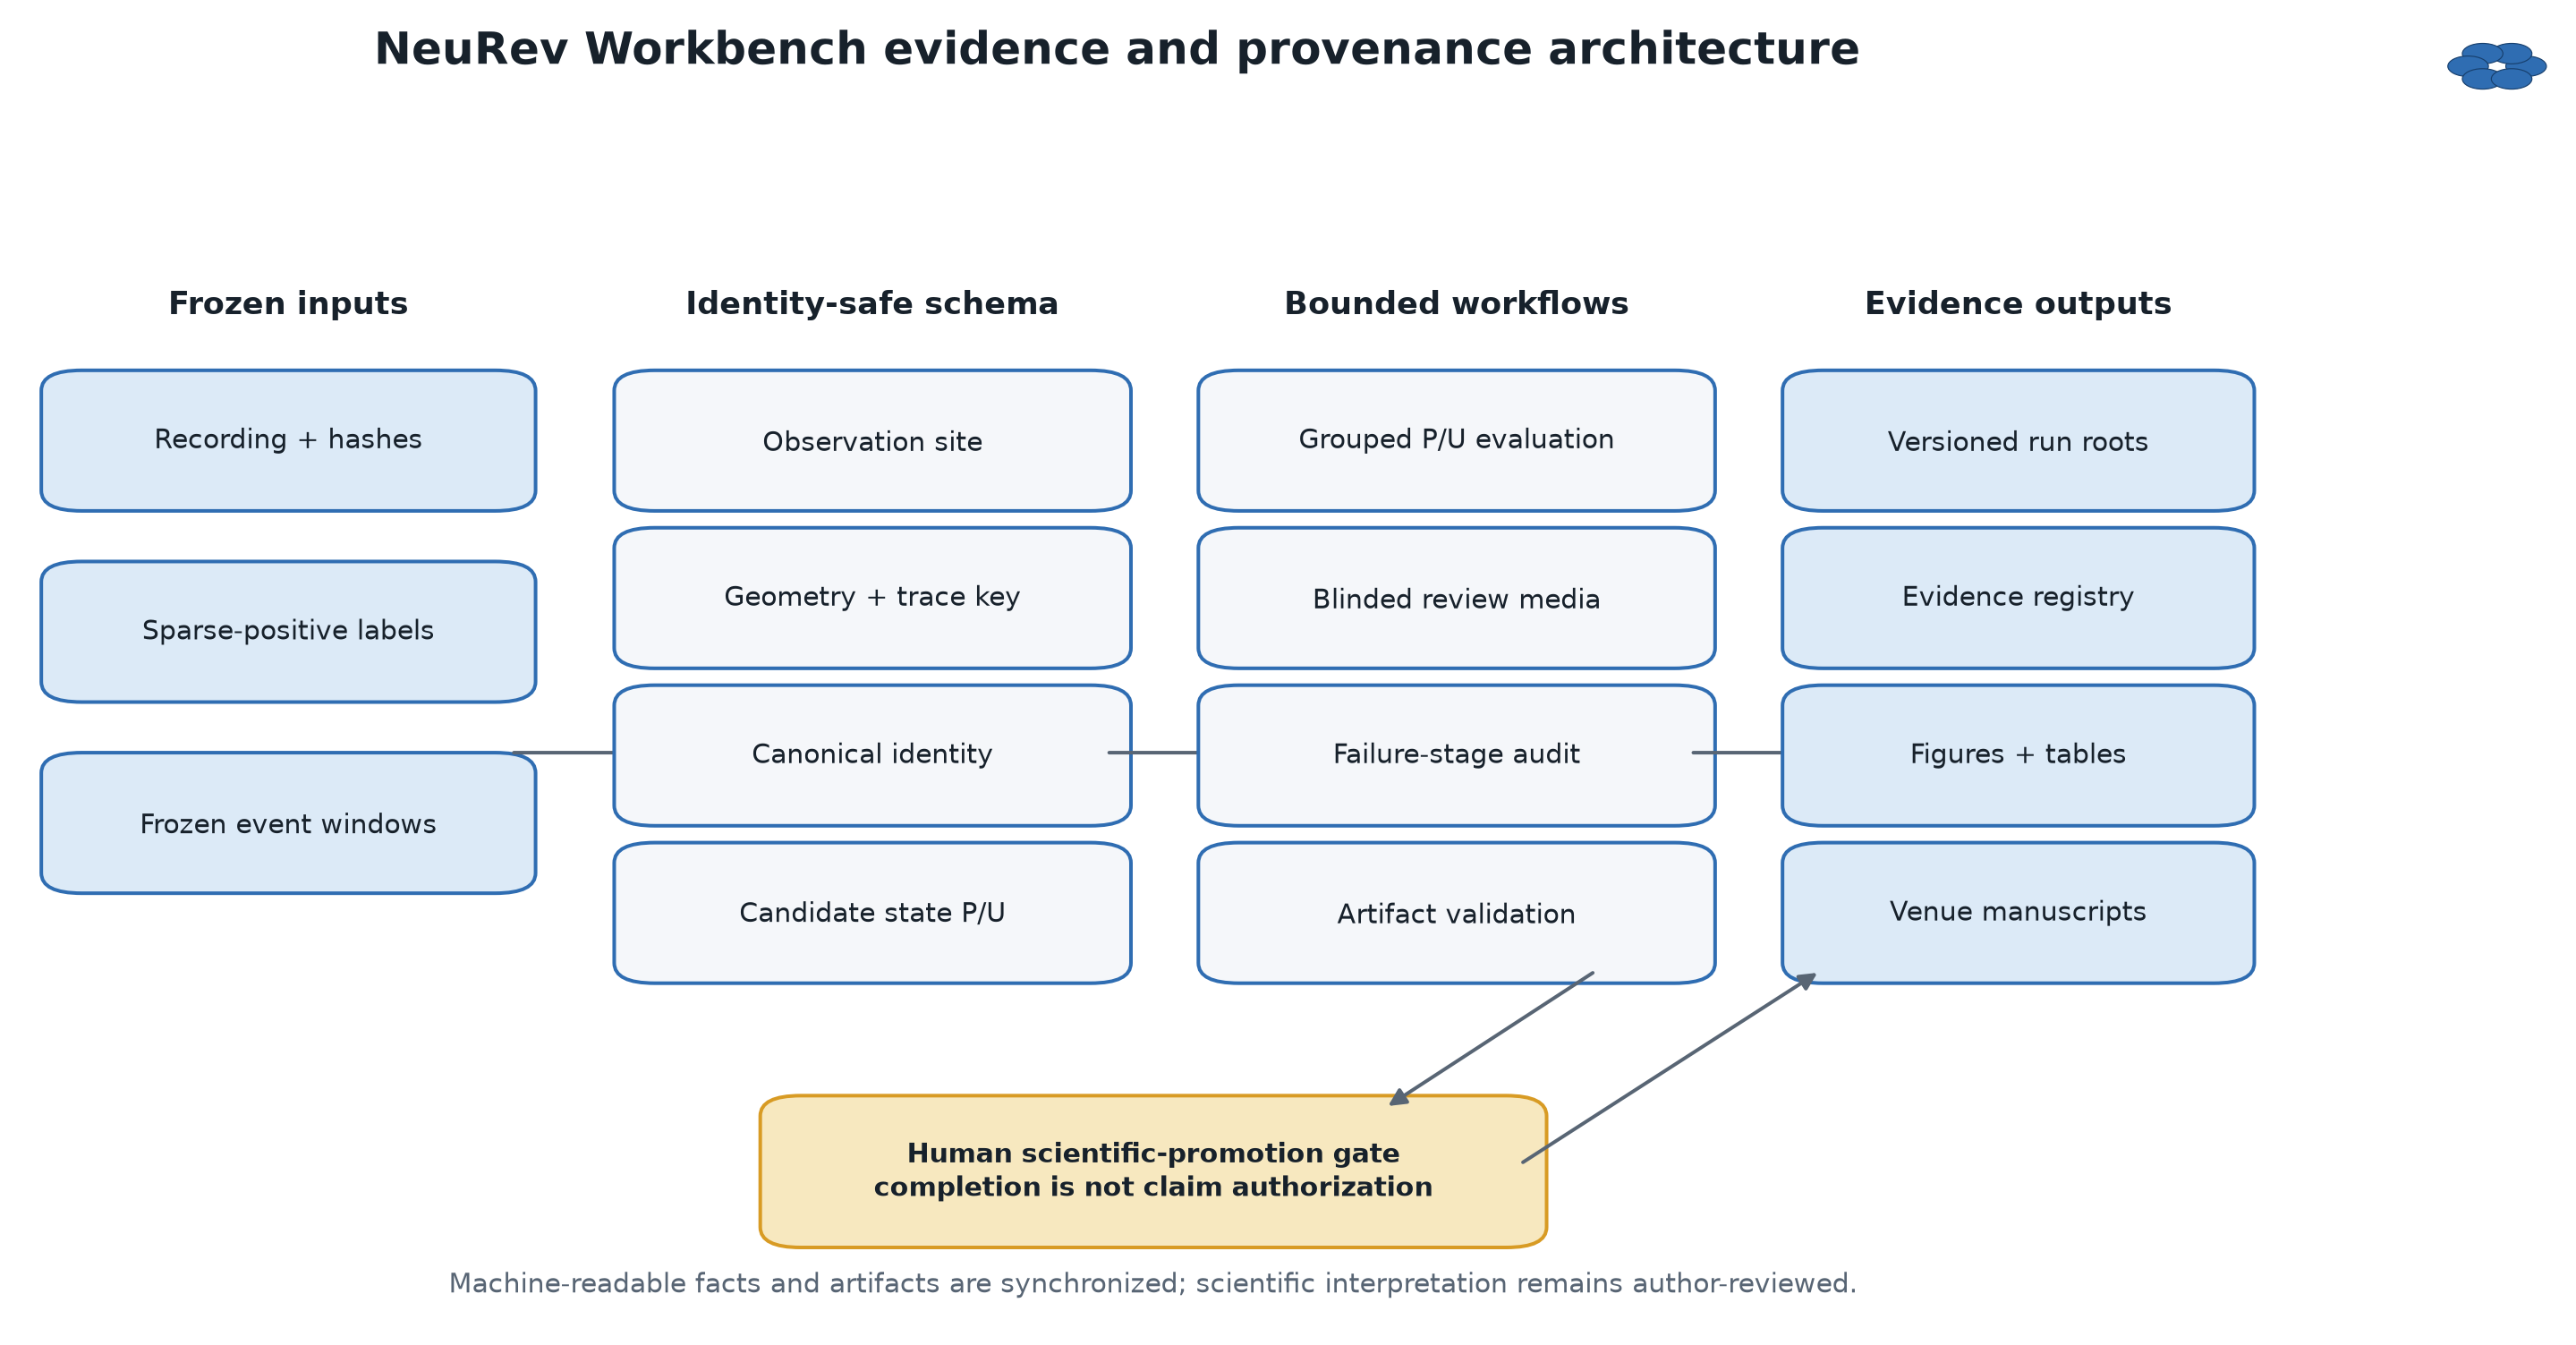
\includegraphics[width=\textwidth]{figures/venue/fig01_neuroinformatics_architecture.png}
  \caption{NeuRev Workbench identity and provenance architecture. Frozen inputs
  enter an identity-safe schema, bounded workflows produce immutable artifacts,
  and compact evidence outputs feed figures and venue manuscripts. Run
  completion and numerical validation do not bypass the human scientific-
  promotion gate.}
  \label{fig:venue-study-design}
\end{figure*}
